\chapter[Introdução]{Introdução}

Ao longo dos anos, agricultores buscaram soluções para o cultivo em ambientes protegidos e seguros. Além disso, houve uma necessidade de produzir em períodos climáticos desfavoráveis, ter o melhor controle do plantio como um todo e realizar o desuso quanto aos agrotóxicos causadores de enfermos. Essas causas, inspirou a realização de muito estudo para proteger o plantio dos dados causados pela natureza e para a não utilização de pesticidas, sendo estes responsáveis por doenças em consumidores. Motivou-se então a criação de um microclima adequado para o cultivo do plantio e tornar o desenvolvimento de hortaliças mais seguro e controlável. 

\section{Contexto}
 
Um grupos de alunos de Engenharia da Universidade de Brasília do Campus do Gama propuseram desenvolver uma estufa hidropônica automatizada, nomeada como Greenhouse, capaz de manter as condições ideais para o cultivo de hortaliças, onde há a permissão do uso de configurações pré-definidas quanto a customização das condições internas, tendo então a disponibilidade do fornecimento de dados ao usuário através de uma interface local, um aplicativo mobile e um sistema
web. O escopo não engloba a produção de plantas que não sejam hortaliças; a produção de hortaliças que não suportam um sistema de hidroponia; o controle da umidade; e a utilização em um ambiente aberto (i.e. outdoor). 

\section{Justificativa}

O objetivo do projeto Greenhouse é fornecer a moradores de casas e apartamentos uma forma automatizada de cultivar hortaliças em suas residências. Isto irá permitir que, mesmo sem uma grande área dedicada, tempo, ou conhecimentos sobre cultivo, os usuários possam cultivar seus próprios produtos orgânicos para consumo próprio.

\section{Escopo do projeto}
 \subsection{Premissas}
  
 \begin{itemize}
 	\item  O produto será utilizado exclusivamente para o cultivo de hortaliças.
 	\item O produto será utilizado exclusivamente em um ambiente fechado (i.e. não será utilizado ao ar livre).
 	\item  O produto estará conectado a uma fonte de água.
 	\item Não serão utilizados pesticidas nas hortaliças cultivadas no produto, ou na água utilizada pelo mesmo.
 \end{itemize}
  
  \subsection{Restrições}
  
  \begin{itemize}
  	\item Irá controlar uma situação de um sistema especificamente hidropônico.
  	\item O produto não poderá ser instalado em um sistema aberto (i.e. outdoor).
  \end{itemize}
                             

\section{Detalhamento do escopo}
\subsection{Projeto}
A equipe Greenhouse pretende contornar as adversidades descritas ao realizar um controle do cultivo, ao constatar a praticidade e despreocupação do usuário final com relação ao desenvolvimento automatizado das hortaliças, além do controle do usuário para as mudanças pertinentes de cada espécie, notificando-o sempre que necessário para que o mesmo esteja ciente do monitoramento do plantio.

O público alvo do projeto são as pessoas preocupadas em produzir o cultivo de hortaliças em um local protegido e em fácil acesso, monitoramento e controle de seu equipamento, sendo este instalado em uma casa, apartamento ou em qualquer local que forneça suas especificações de dimensionamento e que tenha conexão a uma fonte de água.

\subsection{Produto}

O sistema de automatização da estufa irá controlar a temperatura e umidade interna, realizar a abertura automática da gaveta onde se comportará o sistema composto pelas hortaliças e monitorar nível da água, temperatura da água e pH da água.

O sistema funcionará da seguinte forma: o usuário prepara os sachês com substâncias específicas para a germinação, implementa a semente da hortaliça de acordo com as especificações ideais de plantio, informa no sistema web a espécie da hortaliça e acompanha o desenvolvimento da mesma por meio de gráficos e informações de uso disponíveis no sistema web, pois os dados coletados pelos sensores da estufa irá para o servidor web e estará disponível para o monitoramento de todos os dados previamente planejados e o controle de alguns dados específicos, caso não há internet no local de instalação da estufa, os dados estarão empilhados e disponíveis para o acompanhamento quando houver conexão de internet.

A estrutura completa terá dimensões ideias para sua instalação em apartamentos, casas e afins.
\section{Objetivos}

\subsection{Objetivo Geral}

Levando em consideração a dificuldade das pessoas em produzir hortaliças por meio do cultivo residencial, principalmente aquelas que convivem em residências privadas de luz solar e jardinagem, o deferido trabalho propõe a criação de uma estufa hidropônica automatizada dando importância nos aspectos agronômicos para que seja cultivado hortaliças sem dificuldades e que seja realizada a transparência do usuário com relação ao monitoramento e o controle de alguns parâmetros relavantes para o desenvolvimento das hortaliças. 

\subsection{Objetivos Específicos}

A partir das diretrizes acima, o presente trabalho determina que seja desenvolvido os seguintes quesitos a serem desenvolvidos:
	\begin{itemize}
 		\item Produzir uma estrutura composta por um chassi externo isolado que irá conter uma área de cultivo, uma área do reservatório e uma área de iluminação.
 		\item Realizar a comunicação com o sensor DHT22 para umidade relativa do ar e temperatura do ar.
 		\item Realizar a comunicação com o sensor DS18B20 para temperatura da água.
 		\item Realizar a comunicação com o sensor PCF8591 para leitura do PH e Luminosidade a partir de um Conversor A/D.
 		\item Realizar a comunicação d sensores de nível de água por meio de boias.
 		\item Projetar e implementar um sistema que irá realizar a coleta e envio de dados para uma plataforma Web e Mobile por meio de uma Rapberry Pi.
 		\item Projetar e implementar um sistema Web e Mobile.
 		
	\end{itemize}

\section{Metodologia de gerenciamento}

Espaço reservado para Metodologia de gerenciamento.

\subsection{Plano de gerenciamento de comunicação}

Espaço reservado para Plano de gerenciamento de comunicação.

\subsubsection{Organização das reuniões}

Espaço reservado para agendamento organização das reuniões.

\subsubsection{Monitoramento e Controle}


Espaço reservado para Monitoramento e Controle.

\subsection{Plano de gerenciamento de riscos}

Espaço reservado para Plano de gerenciamento de riscos.


\subsection{EAP}

Espaço reservado para EAP.

\begin{figure}[H]
	\centering
%	\includegraphics[width=16cm]{figuras/eap.eps}
%	\caption{EAP - estrutura analítica do projeto} \label{eap}
\end{figure}

\subsection{Cronograma}

Espaço reservado para o cronograma.

\begin{figure}[H]
	\centering
%	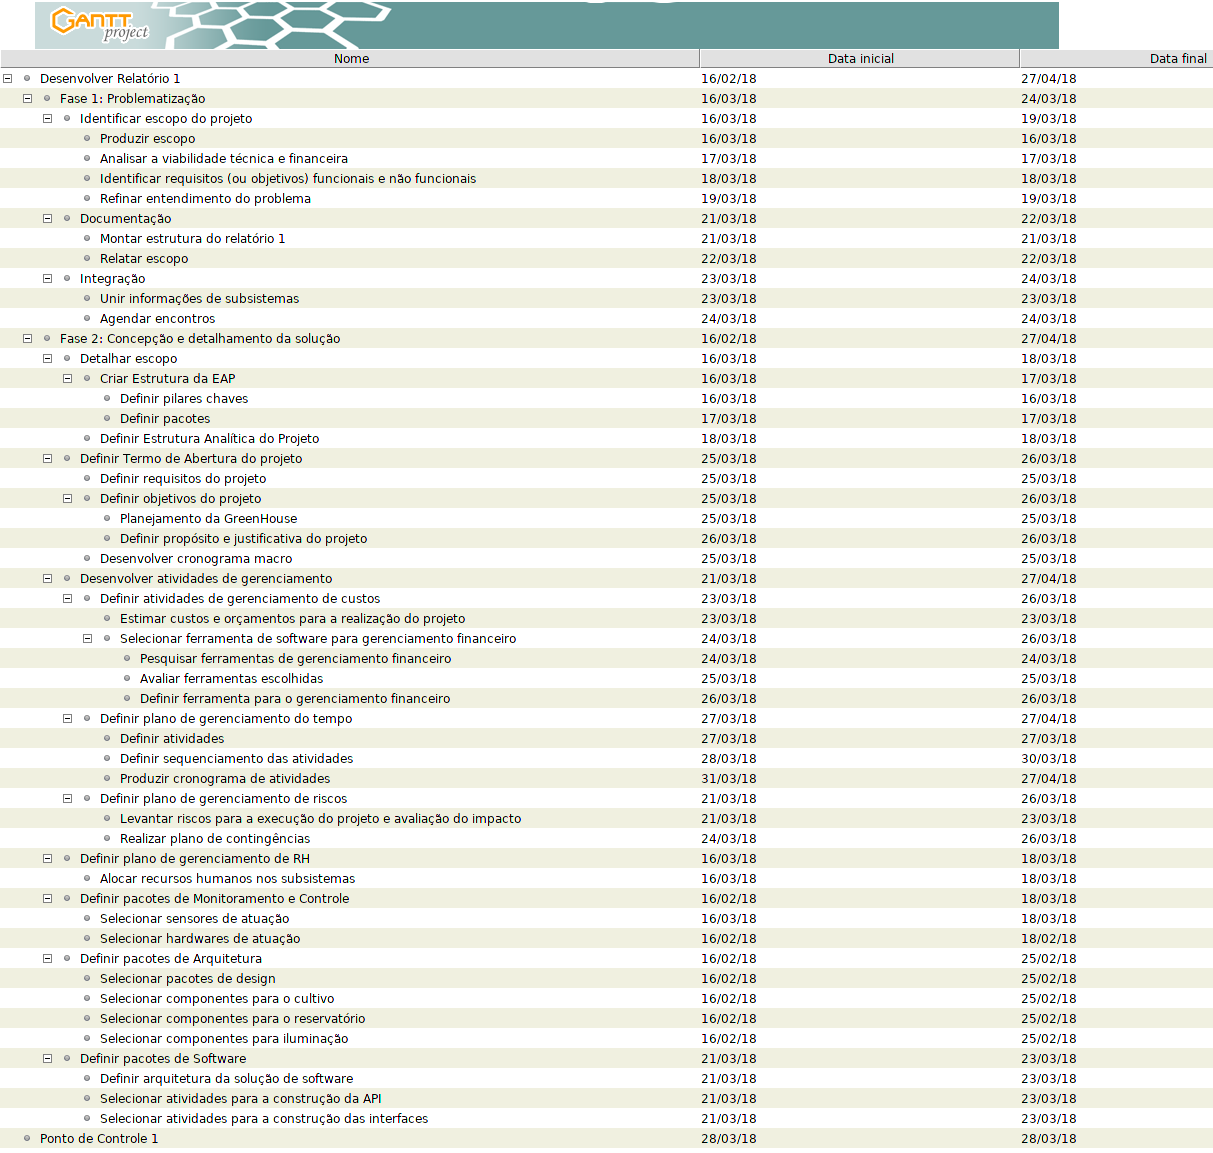
\includegraphics[width=16cm]{figuras/cronograma_1.eps}
	\caption{Cronograma do projeto} \label{cronograma_1}
\end{figure}

\begin{figure}[H]
	\centering
%	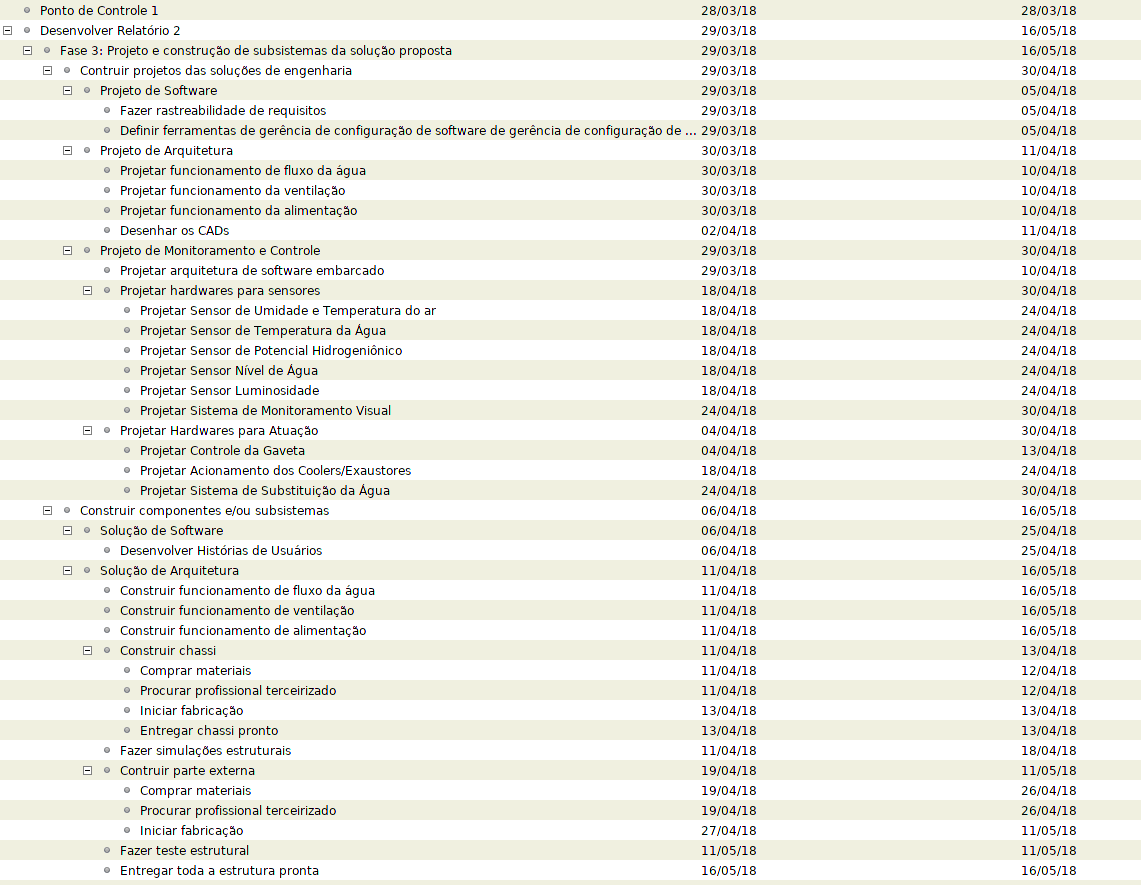
\includegraphics[width=16cm]{figuras/cronograma_2.eps}
	\caption{Cronograma do projeto} \label{cronograma_2}
\end{figure}




